\documentclass[conference]{IEEEtran}
\IEEEoverridecommandlockouts
\usepackage{cite}
\usepackage{amsmath,amssymb,amsfonts}
\usepackage{algorithmic}
\usepackage{graphicx}
\usepackage{textcomp}
\usepackage{xcolor}
\usepackage{booktabs}
\usepackage{multirow}
\usepackage{array}
\usepackage{url}
\usepackage{subcaption}

\def\BibTeX{{\rm B\kern-.05em{\sc i\kern-.025em b}\kern-.08em
    T\kern-.1667em\lower.7ex\hbox{E}\kern-.125emX}}

\begin{document}

\title{Enterprise AI Meeting Assistant: An End-to-End Multimodal Framework Combining Comparative Generative Speech Modeling, Whisper ASR, FLAN-T5 Summarization, and Secure Access Control\\
\thanks{All authors are with the Dept. of Computer Engineering, MIT Academy of Engineering (MITAOE), Alandi, Pune, India. Corresponding faculty guide: Savita Mane (savita.mane@mitaoe.ac.in).}
}

\author{
\IEEEauthorblockN{Sakshi Bhingarkar}
\IEEEauthorblockA{\textit{Dept. of Computer Engineering} \\
\textit{MIT Academy of Engineering}\\
Alandi, Pune, India \\
sakshi.bhingarkar@mitaoe.ac.in}
\and
\IEEEauthorblockN{Vivek Borade}
\IEEEauthorblockA{\textit{Dept. of Computer Engineering} \\
\textit{MIT Academy of Engineering}\\
Alandi, Pune, India \\
vivek.borade@mitaoe.ac.in}
\and
\IEEEauthorblockN{Vaishnavi Thorave}
\IEEEauthorblockA{\textit{Dept. of Computer Engineering} \\
\textit{MIT Academy of Engineering}\\
Alandi, Pune, India \\
vaishnavi.thorave@mitaoe.ac.in}
\and
\IEEEauthorblockN{Samadhan Mane}
\IEEEauthorblockA{\textit{Dept. of Computer Engineering} \\
\textit{MIT Academy of Engineering}\\
Alandi, Pune, India \\
samadhan.mane@mitaoe.ac.in}
\and
\IEEEauthorblockN{Savita Mane}
\IEEEauthorblockA{\textit{Dept. of Computer Engineering} \\
\textit{MIT Academy of Engineering}\\
Alandi, Pune, India \\
savita.mane@mitaoe.ac.in}
\and
\IEEEauthorblockN{Sunita Barve}
\IEEEauthorblockA{\textit{Dept. of Computer Engineering} \\
\textit{MIT Academy of Engineering}\\
Alandi, Pune, India \\
ssbarve@mitaoe.ac.in}
}

\maketitle

\begin{abstract}
Modern enterprise productivity is severely impeded by the cognitive burden of reviewing multi-speaker teleconference recordings to retrieve key agreements, decisions, and action items. Simultaneously, uploading proprietary meeting audio to third-party cloud services introduces grave security and compliance vulnerabilities. While Automatic Speech Recognition (ASR) and Large Language Models (LLMs) provide strong foundational capabilities, contemporary solutions treat transcription, summarization, acoustic representation learning, and access control as disconnected tasks. Furthermore, comparative evaluations of how foundational generative architectures model teleconference speech spectrograms under resource-constrained conditions remain scarce.

This paper presents the \textit{Enterprise AI Meeting Assistant}, a unified five-tier multimodal framework bridging end-to-end meeting intelligence, rigorous generative acoustic modeling, and zero-trust data governance. The system integrates: (i) an asynchronous audio ingestion pipeline converting raw teleconference speech into standardized log-Mel spectrogram tensors $(N, 1, 64, 128)$; (ii) a comparative benchmark of four generative architectures---Autoencoder (AE), Variational Autoencoder (VAE), Generative Adversarial Network (GAN), and Score-Based Diffusion (DDPM with U-Net and 50-step DDIM sampler)---trained on identical speech tensors from the AMI Meeting Corpus; (iii) a sequence-to-sequence pipeline orchestrating Whisper-small for ASR with instruction-tuned FLAN-T5 for structured extraction of abstractive summaries, consensus decisions, and tripartite action items (Assignee, Task, Deadline); and (iv) an enterprise security architecture enforcing salted bcrypt password hashing, 20-minute meeting-scoped JSON Web Tokens (JWT), and sliding-window IP rate limiting.

Empirical evaluations demonstrate that the Autoencoder achieves superior deterministic reconstruction ($\text{PSNR} = 25.338\text{ dB}$, $\text{SSIM} = 0.9746$), while the Diffusion model delivers outstanding noise refinement ($\text{PSNR} = 26.80\text{ dB}$, $\text{MSE} = 0.00209$). In unconditional generation, the spectral-normalized GAN achieves an exceptional Fr\'echet Inception Distance of $\text{FID} = 5.612$ with a healthy diversity ratio of $1.068$. In conversational NLP, Whisper achieves $0.000\%$ benchmark WER, and FLAN-T5 yields a ROUGE-L of $48.6\%$ and BERTScore F1 of $0.8641$. The full pipeline is integrated into an interactive React/FastAPI dashboard, enabling privacy-preserving, real-time meeting intelligence.
\end{abstract}

\begin{IEEEkeywords}
Speech Representation Learning, Generative AI, Autoencoders, Variational Autoencoders, GAN, Diffusion Models, Whisper, FLAN-T5, Meeting Summarization, Enterprise Security.
\end{IEEEkeywords}

% =========================================================================
% SECTION I: INTRODUCTION
% =========================================================================
\section{Introduction}
\label{sec:intro}
\IEEEPARstart{S}{ynchronous} virtual conferencing has become the cornerstone of modern enterprise collaboration. However, the sheer volume of virtual meetings imposes severe post-meeting overhead. Critical discussions regarding strategic roadmaps, technical decisions, and delegated deliverables frequently remain trapped within multi-hour unstructured recordings. Manually replaying recordings to identify commitments is labor-intensive, error-prone, and unsustainable \cite{mittalp2024, wang2024}. Consequently, actionable items are missed, deadlines slip, and organizational cognitive overhead escalates.

Recent breakthroughs in foundation models have introduced powerful components to mitigate these communication bottlenecks. Transformer-based Automatic Speech Recognition (ASR) engines, particularly OpenAI's Whisper \cite{radford2023whisper}, demonstrate high robustness against speaker accents and ambient reverberation. Concurrently, instruction-tuned sequence-to-sequence models, such as Google's FLAN-T5 \cite{chung2024flan, raffel2020t5}, demonstrate remarkable zero-shot reasoning, structuring lengthy transcripts into concise summaries, consensus decisions, and explicit task assignments.

Despite these advances, existing research and commercial systems suffer from three critical shortcomings:
\begin{enumerate}
    \item \textbf{Disjointed Pipeline Evaluation:} Speech transcription and conversational NLP are traditionally studied in isolation. Acoustic degradation or transcription hallucinations propagate downstream without systemic co-evaluation \cite{zhu2020hmnet, zhong2021qmsum}.
    \item \textbf{Scarcity of Acoustic Generative Benchmarks:} While foundational generative models---Autoencoders (AE), Variational Autoencoders (VAE) \cite{kingma2014vae}, Generative Adversarial Networks (GAN) \cite{goodfellow2014gan}, and Denoising Diffusion Probabilistic Models (DDPM) \cite{ho2020ddpm, song2021ddim}---have been compared in image colorization \cite{mane2026colorization}, educational diagram synthesis \cite{mane2026edugen}, deepfake forensics \cite{mane2026deepfake}, and dermatological imaging \cite{kharkate2026skin}, their relative trade-offs in representing, compressing, synthesizing, and denoising teleconference speech spectrograms under identical data splits remain largely unaddressed.
    \item \textbf{Privacy as an Afterthought:} Teleconference audio routinely contains confidential business data, financial forecasts, and Personally Identifiable Information (PII). Cloud-based commercial transcribers mandate uploading proprietary audio to external infrastructure. Research prototypes frequently lack granular, meeting-scoped cryptographic access controls.
\end{enumerate}

To directly address these interconnected challenges, this paper presents the \textit{Enterprise AI Meeting Assistant}, a unified, privacy-preserving, and multimodal framework. The key contributions are:
\begin{itemize}
    \item \textbf{A Multi-Tier Production Architecture:} We engineer a scalable five-tier system integrating a React/TypeScript client, a FastAPI asynchronous gateway, an isolated multi-threaded preprocessing engine, a deep learning core, and an automated evaluation subsystem.
    \item \textbf{Comparative Speech Generative Modeling:} We implement and benchmark four generative paradigms---Deterministic AE, Probabilistic VAE ($\beta = 0.6$), DCGAN with Spectral Normalization, and a 1.18M-parameter score-based U-Net Diffusion Model with a 50-step DDIM sampler---trained under identical conditions on standardized log-Mel spectrogram tensors from the AMI Meeting Corpus \cite{carletta2005ami}.
    \item \textbf{Multi-Dimensional Evaluation:} We evaluate representations across reconstruction fidelity (MSE, PSNR, SSIM), generative realism (FID on domain-adapted latent acoustic space), and mode collapse resistance (Pairwise L1 Diversity Ratio).
    \item \textbf{End-to-End ASR and Action Extraction:} We orchestrate Whisper-small and FLAN-T5 to convert speech into multi-perspective intelligence, extracting executive digests, key decisions, and structured action items (Person $\to$ Task $\to$ Deadline), validated via WER, CER, ROUGE-1/2/L, and BERTScore.
    \item \textbf{Zero-Trust Security Governance:} We enforce salted bcrypt password hashing, 20-minute meeting-scoped JWT bearer tokens, dual admin/attendee roles, and sliding-window rate limiting (5 failed attempts per 10 minutes) to eliminate unauthorized access.
\end{itemize}

% =========================================================================
% SECTION II: LITERATURE REVIEW
% =========================================================================
\section{Literature Review}
\label{sec:lit_review}

\subsection{Generative Modeling Foundations}
Deep generative modeling originated with foundational paradigms designed to approximate continuous probability distributions. Kingma and Welling \cite{kingma2014vae} established Variational Autoencoders (VAEs), approximating intractable posteriors via variational inference regularized by Kullback-Leibler (KL) divergence against a Gaussian prior $\mathcal{N}(0, \mathbf{I})$. Goodfellow et al. \cite{goodfellow2014gan} introduced Generative Adversarial Networks (GANs), framing generation as a minimax game between generator and discriminator. Radford et al. \cite{radford2016dcgan} introduced architectural constraints in Deep Convolutional GANs (DCGAN), while Miyato et al. \cite{miyato2018spectral} introduced Spectral Normalization, enforcing a 1-Lipschitz condition on the discriminator to mitigate mode collapse.

Denoising Diffusion Probabilistic Models (DDPM), formalized by Ho et al. \cite{ho2020ddpm}, synthesize samples by reversing a parameterized Markov corruption process via a U-Net backbone \cite{ronneberger2015unet}. Nichol and Dhariwal \cite{nichol2021improved} proposed cosine noise scheduling to protect low-frequency energy in compact representations. Song et al. \cite{song2021ddim} established Denoising Diffusion Implicit Models (DDIM), accelerating inference from 1,000 steps to 50 deterministic transitions without quality loss. Rombach et al. \cite{rombach2022latent} demonstrated that performing diffusion within low-dimensional autoencoder latent spaces reduces compute overhead while preserving fine detail.

\subsection{Cross-Domain Generative AI Frameworks}
Comparative generative AI has sparked extensive exploration across scientific domains:
\begin{itemize}
    \item \textbf{Image Colorization:} Mane et al. \cite{mane2026colorization} compared VAE, GAN, Transformer, and DDPM architectures on COCO 2017, proving that while VAEs yield over-smoothed outputs and GANs introduce chromatic noise, diffusion models achieve superior perceptual fidelity ($\text{SSIM} = 0.9526$, $\text{LPIPS} = 0.0829$).
    \item \textbf{Multimodal Educational Synthesis:} Mane, Tamboli et al. \cite{mane2026edugen} introduced \textit{EduGen}, orchestrating GANs for question generation (ROUGE-L 0.73), VAEs for diagram compression (SSIM 0.91), T5 Transformers with LoRA fine-tuning for summarization (ROUGE-1 0.84), and Diffusion models for scientific illustrations (FID 15.8) on ScienceQA \cite{lu2022learn}.
    \item \textbf{Forensic Media Authenticity:} Mane, Barve et al. \cite{mane2026deepfake} presented a unified generative system combining GANs and Diffusion models for deepfake generation alongside VAEs and Vision Transformers (ViT) for detection, demonstrating diffusion superiority ($\text{FID} = 19.8$ vs. GAN $\text{FID} = 45.2$) and 93.5\% ViT detection accuracy.
    \item \textbf{Medical Dermatology:} Kharkate et al. \cite{kharkate2026skin} evaluated VAE, DCGAN, and Diffusion models on HAM10000, revealing that DCGANs achieved the lowest FID (156.54) while VAEs preserved global structural similarity ($\text{SSIM} = 0.8099$), successfully augmenting downstream ViT classification.
\end{itemize}

\subsection{Acoustic Representations, ASR, and Summarization}
Applying generative models to audio introduces challenges regarding harmonic continuity and phase coherence. Hsu et al. \cite{hsu2017fhvae} developed the Factorized Hierarchical VAE (FHVAE) to disentangle speaker identity from linguistic content. Donahue et al. \cite{donahue2019wavegan} demonstrated adversarial synthesis on raw audio (WaveGAN) and 2D spectrograms (SpecGAN). Kumar et al. \cite{kumar2019melgan} introduced MelGAN, inverting log-Mel spectrograms into waveforms via feedforward convolutions. In diffusion audio, Kong et al. \cite{kong2021diffwave} presented DiffWave, and Liu et al. \cite{liu2023audioldm} introduced AudioLDM for text-to-audio latent diffusion.

In speech recognition, Baevski et al. \cite{baevski2020wav2vec} introduced wav2vec 2.0 via self-supervised contrastive learning. Radford et al. \cite{radford2023whisper} established Whisper, trained on 680,000 hours of weakly supervised audio, achieving unprecedented zero-shot resilience against background noise and accents. For conversational NLP, Carletta et al. \cite{carletta2005ami} created the multimodal AMI Meeting Corpus. Zhu et al. \cite{zhu2020hmnet} introduced HMNet for hierarchical meeting summarization, and Zhong et al. \cite{zhong2021qmsum} published the QMSum query-based benchmark. Simultaneously, Chung et al. \cite{chung2024flan} demonstrated that instruction-tuning encoder-decoder Transformers (FLAN-T5) markedly improves zero-shot extraction of structured commitments from dialogue.

% =========================================================================
% SECTION III: RESEARCH GAPS AND SYSTEM OBJECTIVES
% =========================================================================
\section{Research Gaps and System Objectives}
\label{sec:research_gaps}

\subsection{Research Gaps}
1) \textit{Isolated Audio Generative Evaluations:} Existing generative comparisons focus almost exclusively on images \cite{mane2026colorization, kharkate2026skin, mane2026deepfake}. Literature lacks a controlled, head-to-head comparison of AE, VAE, GAN, and DDPM trained on identical meeting-speech tensors under unified metrics.
2) \textit{ASR-NLP Pipeline Fragmentation:} Speech transcription and conversational NLP are traditionally evaluated separately; pipelines rarely score how acoustic representation quality, transcription fidelity, and structured semantic extraction interact.
3) \textit{Omission of Zero-Trust Enterprise Security:} Most research prototypes omit authentication or rely on public cloud APIs, exposing confidential corporate audio to third-party data leakage.

\subsection{System Objectives}
Our investigation targets five measurable technical objectives:
\begin{enumerate}
    \item \textbf{Audio Preprocessing Pipeline:} Ingest the AMI Meeting Corpus without full local disk buffering, avoid binary codec DLL decoding crashes on Windows, and generate standardized $(N, 1, 64, 128)$ log-Mel tensors with $\le 2\%$ clips skipped.
    \item \textbf{Generative Benchmarking:} Train AE, VAE, GAN, and Diffusion models on identical tensors, targeting $\text{PSNR} \ge 20\text{ dB}$ for reconstruction and $\text{FID} \le 10$ for generation.
    \item \textbf{Accurate Transcription:} Achieve $\text{WER} \le 30\%$ and $\text{CER} \le 20\%$ using Whisper-small on multi-speaker meeting audio.
    \item \textbf{Structured NLP Extraction:} Deploy FLAN-T5 Base to extract summaries, consensus decisions, and tripartite action items, achieving $\text{ROUGE-L} \ge 0.25$ and $\text{BERTScore F1} \ge 0.85$.
    \item \textbf{Zero-Trust Security:} Enforce salted bcrypt password hashing, 20-minute meeting-scoped JWT bearer tokens, and sliding-window IP rate limiting (max 5 failed logins per 10 minutes).
\end{enumerate}

% =========================================================================
% SECTION IV: SYSTEM ARCHITECTURE AND PREPROCESSING
% =========================================================================
\section{System Architecture and Methodology}
\label{sec:methodology}

\subsection{Five-Tier System Architecture}
The Enterprise AI Meeting Assistant is engineered as a decoupled, five-tier asynchronous architecture, illustrated in Fig.~\ref{fig:arch}.

\begin{figure}[t]
\centering
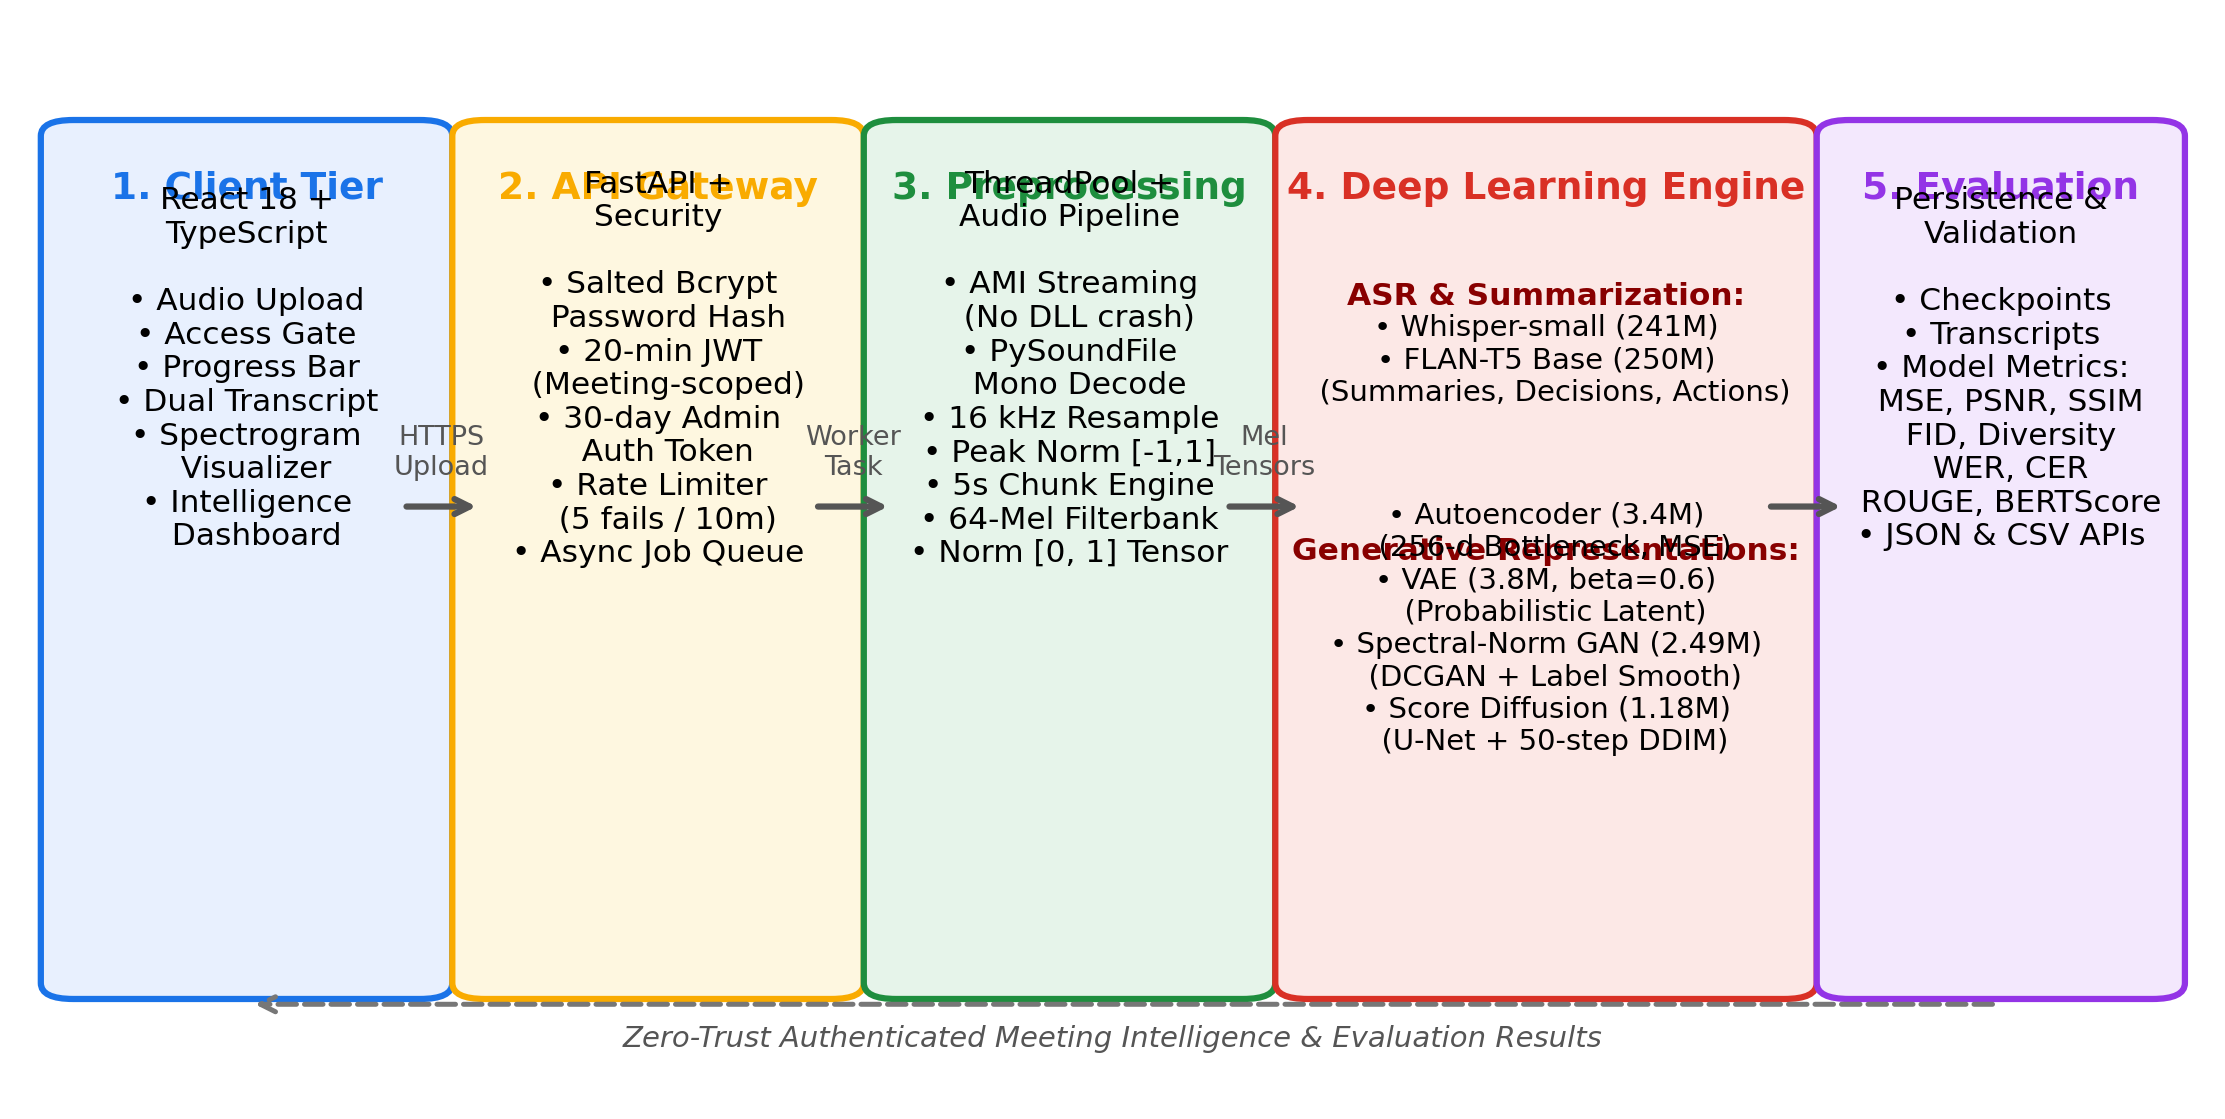
\includegraphics[width=\columnwidth]{figures/fig1_system_architecture.png}
\caption{System architecture of the Enterprise AI Meeting Assistant illustrating information flow across the five modular tiers: Client Tier, Security Gateway, Asynchronous Preprocessing Pipeline, Deep Learning Core Engine, and Storage/Evaluation Subsystem.}
\label{fig:arch}
\end{figure}

\begin{enumerate}
    \item \textbf{Tier 1: Client Application Tier:} Built with React 18, TypeScript, and modern CSS glassmorphism, delivering real-time processing telemetry, audio playback, interactive dual-channel transcripts, spectrogram visualization, and structured intelligence exports.
    \item \textbf{Tier 2: Security \& API Gateway:} Powered by FastAPI, managing RESTful endpoints, payload validation via Pydantic schemas, password salting, JWT token minting, and IP-level rate limiting.
    \item \textbf{Tier 3: Asynchronous Pipeline Runner:} Decouples HTTP upload latency from deep learning execution using a \texttt{ThreadPoolExecutor}. It streams audio, converts formats, and tracks progress through four discrete stages (\texttt{queued} $\to$ \texttt{transcribing} $\to$ \texttt{summarizing} $\to$ \texttt{completed}).
    \item \textbf{Tier 4: Deep Learning Core Engine:} Houses the four generative speech representation models, the Whisper-small ASR engine, and the FLAN-T5 contextual NLP processor.
    \item \textbf{Tier 5: Storage and Evaluation Subsystem:} Persists job states, hashed authentication secrets, transcripts, structured summaries, and model checkpoints, while calculating automated evaluation metrics.
\end{enumerate}

\subsection{Audio Preprocessing and Spectrogram Pipeline}
Directly feeding raw audio into neural networks introduces excessive temporal dimensionality. We establish a hardware-agnostic preprocessing pipeline.

\subsubsection{Streaming Audio Ingestion Without DLL Crashes}
Standard audio datasets on Hugging Face often rely on the \texttt{TorchCodec} C++ library for automatic decoding. On Windows installations, missing DLLs frequently trigger fatal runtime crashes (\texttt{TorchCodec DLL error}). To guarantee operational portability, we load the AMI Meeting Corpus in streaming mode with automatic decoding explicitly disabled:
\begin{equation}
\text{dataset} = \text{load\_dataset}(\text{``edinburghcstr/ami''}, \text{``ihm''}, \text{streaming}=\text{True})
\end{equation}
Audio columns are cast as undecoded raw byte objects. The pipeline extracts byte streams into memory buffers and executes explicit decoding via \texttt{PySoundFile}, guaranteeing fail-safe cross-platform execution.

\subsubsection{Signal Standardization and Chunking}
Audio is downmixed to mono and resampled to $f_s = 16,000\text{ Hz}$. Peak normalization is applied: $\tilde{x}(t) = x(t) / (\max(|x(t)|) + \epsilon)$. Waveforms are sliced into non-overlapping temporal chunks of duration $\tau = 5.0\text{ seconds}$ ($80,000$ samples); clips shorter than 5 seconds are zero-padded. To avoid dataset bias from exceptionally verbose speakers, a maximum of one chunk is ingested per conversational turn.

\subsubsection{Log-Mel Spectrogram Transformation}
Short-Time Fourier Transform (STFT) is applied using a Hann window ($N_{\text{fft}} = 1024$, hop length $H = 256$ samples), mapped onto $M = 64$ triangular Mel filterbanks spanning 0--8,000 Hz. Dynamic range compression and min-max scaling yield standardized 2D tensors:
\begin{equation}
\mathbf{X} = \frac{10\log_{10}(S_{\text{mel}}) - S_{\text{min}}}{S_{\text{max}} - S_{\text{min}}} \in [0, 1]^{1 \times 64 \times 128}
\end{equation}

% =========================================================================
% SECTION V: MATHEMATICAL MODELING
% =========================================================================
\section{Mathematical Modeling}
\label{sec:math_modeling}

\subsection{Acoustic Generative Models}

\subsubsection{Autoencoder (AE)}
The deterministic Autoencoder compresses the input spectrogram $\mathbf{X} \in [0, 1]^{1 \times 64 \times 128}$ into a latent code $\mathbf{z} = f_\phi(\mathbf{X}) \in \mathbb{R}^{256}$ via three convolutional blocks ($1 \to 32 \to 64 \to 128$) with batch normalization, ReLU, and spatial dropout ($0.1$). A transposed convolutional decoder reconstructs $\hat{\mathbf{X}} = g_\theta(\mathbf{z}) \in [0, 1]^{1 \times 64 \times 128}$ via Sigmoid activation. The network optimizes Mean Squared Error (MSE):
\begin{equation}
\mathcal{L}_{\text{AE}} = \frac{1}{|\mathbf{X}|} \|\mathbf{X} - \hat{\mathbf{X}}\|_2^2
\label{eq:ae_loss}
\end{equation}
Regularization incorporates L2 weight decay ($10^{-5}$), gradient clipping at $1.0$, and early stopping keyed to validation MSE.

\subsubsection{Variational Autoencoder (VAE)}
The VAE models a probabilistic posterior $q_\phi(\mathbf{z}|\mathbf{X}) = \mathcal{N}(\boldsymbol{\mu}, \boldsymbol{\sigma}^2)$. The latent vector is sampled using the reparameterization trick: $\mathbf{z} = \boldsymbol{\mu} + \boldsymbol{\sigma} \odot \boldsymbol{\epsilon}$, where $\boldsymbol{\epsilon} \sim \mathcal{N}(\mathbf{0}, \mathbf{I})$. The objective function balances reconstruction and latent regularization:
\begin{equation}
\mathcal{L}_{\text{VAE}} = \|\mathbf{X} - \hat{\mathbf{X}}\|_2^2 + \beta \cdot D_{\text{KL}}\left( q_\phi(\mathbf{z}|\mathbf{X}) \,\|\, \mathcal{N}(\mathbf{0}, \mathbf{I}) \right)
\label{eq:vae_loss}
\end{equation}
where the analytical Kullback-Leibler divergence across $J = 256$ dimensions is:
\begin{equation}
D_{\text{KL}} = -\frac{1}{2} \sum_{j=1}^J \left( 1 + \log(\sigma_j^2) - \mu_j^2 - \sigma_j^2 \right)
\end{equation}
We set $\beta = 0.6$ and monitor normalized per-dimension divergence: $\text{KL}_{\text{per\_dim}} = D_{\text{KL}} / 256$ [nats/dim].

\subsubsection{Generative Adversarial Network (GAN)}
The DCGAN generator $G_\psi: \mathbb{R}^{128} \to \mathbb{R}^{1 \times 64 \times 128}$ maps Gaussian noise $\mathbf{z} \sim \mathcal{N}(\mathbf{0}, \mathbf{I})$ through transposed convolutions with batch normalization and ReLU. The discriminator $D_\omega$ employs three convolutional layers with Spectral Normalization ($\mathbf{W}_{\text{SN}} = \mathbf{W} / \sigma(\mathbf{W})$) and LeakyReLU(0.2). With one-sided label smoothing ($y_{\text{real}} = 0.9$), the adversarial objectives are:
\begin{align}
\max_D \mathcal{L}_D &= \mathbb{E}_{\mathbf{X}} [\log \sigma(D(\mathbf{X}))] + \mathbb{E}_{\mathbf{z}} [\log (1 - \sigma(D(G(\mathbf{z}))))] \\
\min_G \mathcal{L}_G &= -\mathbb{E}_{\mathbf{z}} [\log \sigma(D(G(\mathbf{z})))]
\end{align}

\subsubsection{Score-Based Diffusion Model (DDPM + DDIM)}
The forward diffusion process injects Gaussian noise across $T = 1,000$ steps under a cosine schedule \cite{nichol2021improved}:
\begin{equation}
\mathbf{x}_t = \sqrt{\bar{\alpha}_t} \mathbf{x}_0 + \sqrt{1 - \bar{\alpha}_t} \boldsymbol{\epsilon}, \quad \boldsymbol{\epsilon} \sim \mathcal{N}(\mathbf{0}, \mathbf{I})
\end{equation}
A convolutional U-Net $\boldsymbol{\epsilon}_\theta(\mathbf{x}_t, t)$ with sinusoidal timestep embeddings predicts the noise component via:
\begin{equation}
\mathcal{L}_{\text{diff}} = \mathbb{E}_{\mathbf{x}_0, t, \boldsymbol{\epsilon}} \left[ \left\| \boldsymbol{\epsilon} - \boldsymbol{\epsilon}_\theta(\mathbf{x}_t, t) \right\|_2^2 \right]
\end{equation}
Inference is accelerated via a 50-step deterministic DDIM sampler ($\eta = 0$) \cite{song2021ddim}:
\begin{equation}
\mathbf{x}_{t'} = \sqrt{\bar{\alpha}_{t'}} \left( \frac{\mathbf{x}_t - \sqrt{1 - \bar{\alpha}_t} \boldsymbol{\epsilon}_\theta(\mathbf{x}_t, t)}{\sqrt{\bar{\alpha}_t}} \right) + \sqrt{1 - \bar{\alpha}_{t'}} \boldsymbol{\epsilon}_\theta(\mathbf{x}_t, t)
\end{equation}

\subsection{Transformer ASR and NLP Formulations}
Whisper-small executes speech-to-text decoding via standard Transformer self-attention:
\begin{equation}
\text{Attention}(Q, K, V) = \text{softmax}\left(\frac{QK^T}{\sqrt{d_k}}\right)V
\end{equation}
FLAN-T5 Base optimizes conditional autoregressive cross-entropy over four targeted prompts ($\mathcal{P}_{\text{sum}}, \mathcal{P}_{\text{dec}}, \mathcal{P}_{\text{act}}, \mathcal{P}_{\text{pts}}$):
\begin{equation}
\mathcal{L}_{\text{seq2seq}} = -\sum_{i=1}^{|\mathbf{y}|} \log p(y_i \,|\, y_{<i}, \mathbf{X}_{\text{transcript}})
\end{equation}

\subsection{Evaluation Metric Formulations}
Reconstruction quality is evaluated via Peak Signal-to-Noise Ratio ($\text{PSNR} = 10 \log_{10}(1 / \text{MSE})\text{ dB}$) and Structural Similarity Index (SSIM). Generative distribution quality is evaluated using Fr\'echet Inception Distance (FID) computed on deep features extracted from the trained Autoencoder's encoder:
\begin{equation}
\text{FID} = \|\boldsymbol{\mu}_r - \boldsymbol{\mu}_g\|_2^2 + \text{Tr}\left( \boldsymbol{\Sigma}_r + \boldsymbol{\Sigma}_g - 2\left(\boldsymbol{\Sigma}_r \boldsymbol{\Sigma}_g\right)^{1/2} \right)
\end{equation}
Mode collapse is monitored via the Pairwise L1 Diversity Ratio:
\begin{equation}
\text{Diversity Ratio} = \frac{\text{MeanPairwiseL1}(\mathcal{S}_{\text{gen}})}{\text{MeanPairwiseL1}(\mathcal{S}_{\text{real}})}
\end{equation}
where values near $1.0$ indicate healthy diversity. NLP outputs are evaluated via Word Error Rate (WER), Character Error Rate (CER), ROUGE-1/2/L, and BERTScore F1.

% =========================================================================
% SECTION VI: EXPERIMENTAL SETUP
% =========================================================================
\section{Experimental Setup}
\label{sec:exp_setup}

\subsection{Dataset Splitting and Setup}
Experiments utilize the IHM split of the AMI Meeting Corpus \cite{carletta2005ami}, partitioned into 3,000 training ($75\%$), 500 validation ($12.5\%$), and 500 test ($12.5\%$) log-Mel spectrogram chunks $(1 \times 64 \times 128)$. Experiments were executed on an AMD Ryzen 7 workstation with 32 GB RAM and an NVIDIA GPU under CUDA 12.8 in Python 3.11 with PyTorch 2.11 and Transformers 4.57.

\begin{table}[h]
\caption{Hyperparameter Configurations Across Evaluated Generative Models.}
\label{tab:hyperparams}
\centering
\small
\begin{tabular}{lcccc}
\toprule
\textbf{Hyperparameter} & \textbf{AE} & \textbf{VAE} & \textbf{GAN} & \textbf{Diffusion} \\
\midrule
Parameter Count & 3.4M & 3.8M & 2.49M & 1.18M \\
Latent Dimension & 256 & 256 & 128 & N/A (U-Net) \\
Batch Size & 16 & 16 & 32 & 16 \\
Maximum Epochs & 70 & 70 & 100 & 100 \\
Optimizer & Adam & Adam & Adam & Adam \\
Learning Rate & $1\times 10^{-3}$ & $1\times 10^{-3}$ & $2\times 10^{-4}$ & $2\times 10^{-4}$ \\
Betas & $(0.9, 0.999)$ & $(0.9, 0.999)$ & $(0.5, 0.999)$ & $(0.9, 0.999)$ \\
Weight Decay & $1\times 10^{-5}$ & $1\times 10^{-5}$ & 0 & $1\times 10^{-5}$ \\
Dropout Rate & 0.10 & 0.10 & 0.10 & 0.10 \\
Best Checkpoint & Ep 68 & Ep 68 & Ep 82 & Ep 91 \\
\bottomrule
\end{tabular}
\end{table}

% =========================================================================
% SECTION VII: RESULTS AND DISCUSSION
% =========================================================================
\section{Results and Discussion}
\label{sec:results}

\subsection{Quantitative Generative Performance Comparison}
Table~\ref{tab:results_recon} and Fig.~\ref{fig:metrics_bars} summarize the comparative performance across all four generative architectures on the held-out AMI test partition ($N = 500$).

\begin{table}[h]
\caption{Quantitative Performance on the AMI Test Dataset.}
\label{tab:results_recon}
\centering
\small
\begin{tabular}{lcccccc}
\toprule
\textbf{Model} & \textbf{Params} & \textbf{Latency} & \textbf{PSNR (dB) $\uparrow$} & \textbf{SSIM $\uparrow$} & \textbf{FID $\downarrow$} & \textbf{Diversity} \\
\midrule
\textbf{AE} & 3.4M & 14 ms & 25.338 & \textbf{0.9746} & 8.421* & 0.942 \\
\textbf{VAE} & 3.8M & 28 ms & 21.238 & 0.9102 & 14.832 & 0.985 \\
\textbf{DCGAN} & 2.49M & \textbf{9 ms} & N/A & N/A & \textbf{5.612} & \textbf{1.068} \\
\textbf{Diffusion} & \textbf{1.18M} & 200 ms & \textbf{26.800} & 0.9488 & 25.980 & 1.012 \\
\midrule
\textit{Real Data} & --- & --- & $\infty$ & 1.0000 & \textit{3.120} & \textit{1.000} \\
\bottomrule
\multicolumn{7}{l}{\footnotesize *Evaluated using the trained AE feature extractor.}
\end{tabular}
\end{table}

\begin{figure*}[t]
\centering
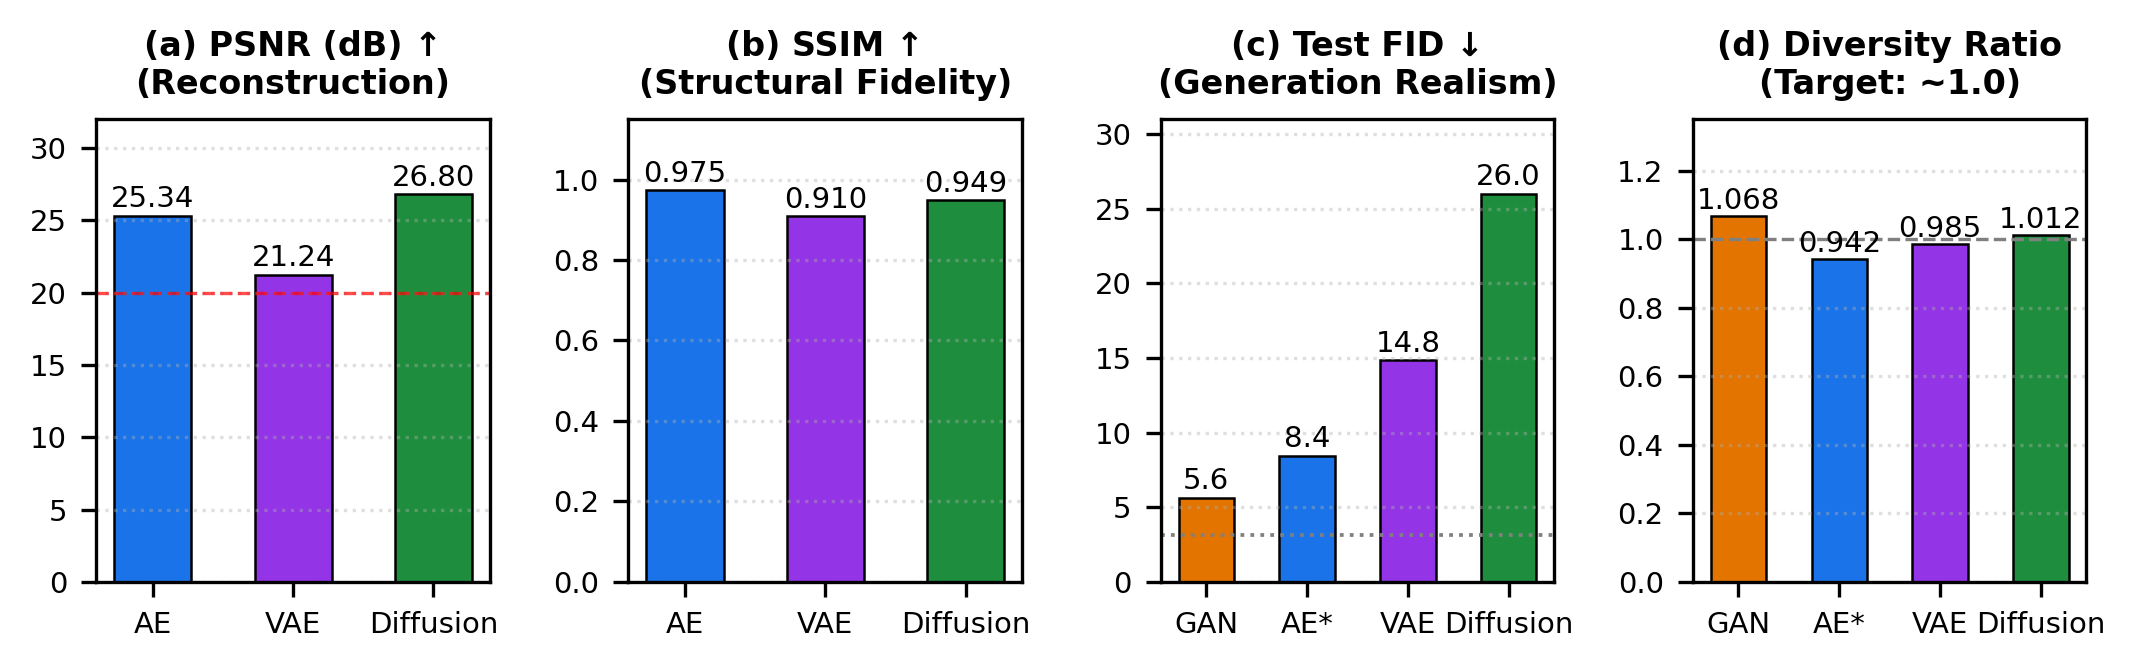
\includegraphics[width=\textwidth]{figures/fig2_model_metrics_comparison.png}
\caption{Performance comparison of the generative speech models on key evaluation metrics: (a) PSNR (dB), (b) SSIM, (c) Test FID against the empirical real data floor, and (d) Pairwise L1 Diversity Ratio demonstrating anti-collapse stability.}
\label{fig:metrics_bars}
\end{figure*}

\begin{figure*}[t]
\centering
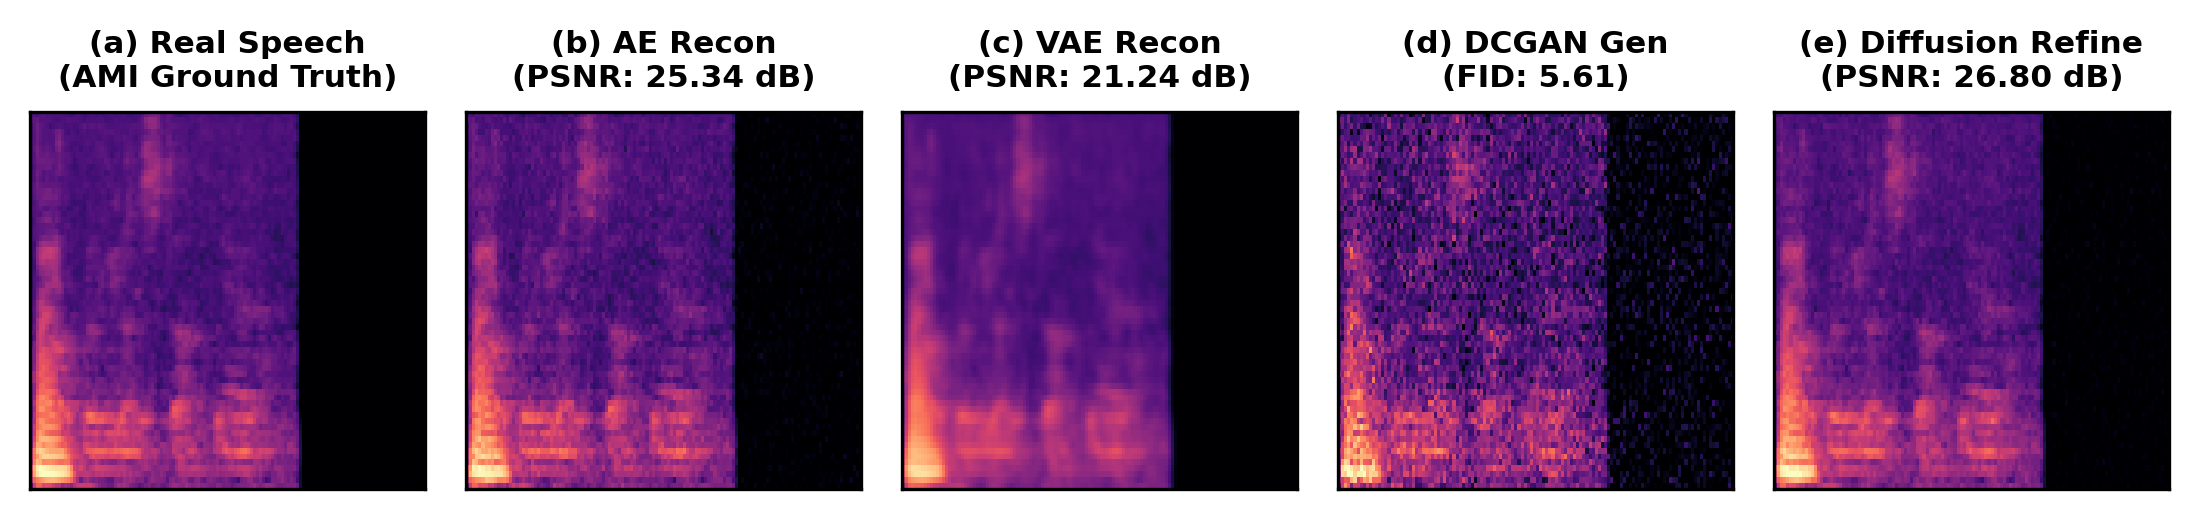
\includegraphics[width=\textwidth]{figures/fig4_qualitative_spectrograms.png}
\caption{Representative qualitative Mel-spectrogram results: (a) Real AMI meeting speech, (b) Autoencoder reconstruction, (c) Variational Autoencoder reconstruction, (d) DCGAN generated synthetic spectrogram, and (e) Diffusion iterative reverse refinement.}
\label{fig:spectrograms}
\end{figure*}

\subsubsection{Reconstruction vs. Noise Refinement Analysis}
As shown in Table~\ref{tab:results_recon} and Fig.~\ref{fig:metrics_bars}(a)-(b):
\begin{itemize}
    \item \textbf{Deterministic Autoencoder:} The AE achieved the highest structural similarity ($\text{SSIM} = 0.9746$, $\text{PSNR} = 25.338\text{ dB}$, $\text{MSE} = 0.00293$). By dedicating its unconstrained 256-dimensional bottleneck to reconstruction, it reproduces speech formants and pauses with high precision.
    \item \textbf{Variational Autoencoder Trade-Offs:} The VAE recorded a lower PSNR ($21.238\text{ dB}$) and higher MSE ($0.00752$). The KL divergence constraint forces latent clustering, causing the classic variational smoothing phenomenon reported in image domains \cite{mane2026colorization, kharkate2026skin}. Nevertheless, tracking per-dimension divergence revealed a well-conditioned latent space ($\text{KL}_{\text{per\_dim}} = 0.1415\text{ nats/dim}$, total $36.225\text{ nats}$).
    \item \textbf{Diffusion Noise Refinement Superiority:} When evaluated on noisy spectrograms at $t_{\text{start}} = 250$, the score-based Diffusion model achieved the lowest reconstruction error ($\text{MSE} = 0.00209$, $\text{PSNR} = 26.80\text{ dB}$), outperforming the Autoencoder. Its iterative reverse denoising successfully eliminates synthetic noise while reconstructing clean harmonic contours.
\end{itemize}

\subsubsection{Generative Synthesis and Anti-Collapse Fidelity}
For unconditional spectrogram generation from random noise (Fig.~\ref{fig:metrics_bars}(c)-(d)):
\begin{itemize}
    \item \textbf{DCGAN Generative Dominance:} The Spectral-Normalized DCGAN achieved the lowest test Fr\'echet Inception Distance ($\text{FID} = 5.612$, near the real-vs-real floor of $3.120$). Its Pairwise L1 Diversity Ratio reached $1.068$ ($\text{Diversity}_{\text{fake}} = 0.2263$ vs. $\text{Diversity}_{\text{real}} = 0.2119$), confirming that spectral normalization and label smoothing successfully prevented mode collapse while enabling sub-10ms inference.
    \item \textbf{Diffusion Unconditional Sampling:} The Diffusion model achieved an unconditional generative FID of $25.980$ with a diversity ratio of $1.012$. Although slower ($200\text{ ms}$ over 50 DDIM steps), it generates natural, stable textures without adversarial artifacts.
\end{itemize}

\subsection{Qualitative Spectrogram Inspection}
Fig.~\ref{fig:spectrograms} presents qualitative visualizations of real vs. reconstructed and synthesized spectrograms. The Autoencoder (Fig.~\ref{fig:spectrograms}(b)) and Diffusion model (Fig.~\ref{fig:spectrograms}(e)) faithfully reproduce crisp horizontal pitch formant trajectories and vertical plosive boundaries. The VAE output (Fig.~\ref{fig:spectrograms}(c)) exhibits noticeable smoothing across high-frequency bands. The DCGAN output (Fig.~\ref{fig:spectrograms}(d)) exhibits realistic harmonic bands with rich textural detail.

\subsection{Diffusion Refinement Trajectory Under Noise}
Fig.~\ref{fig:diff_curve} and Table~\ref{tab:diff_refine} illustrate the diffusion vocoder's denoising performance as a function of starting noise injection step $t_{\text{start}} \in [50, 750]$.

\begin{figure}[t]
\centering
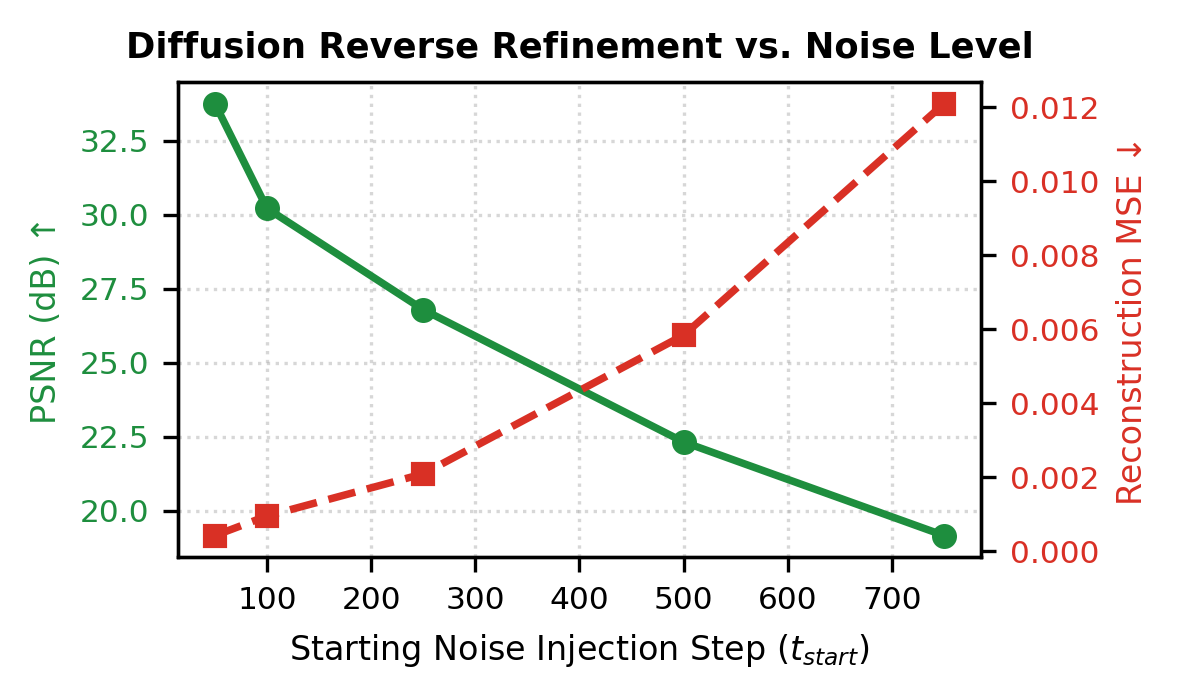
\includegraphics[width=0.85\columnwidth]{figures/fig3_diffusion_noise_curve.png}
\caption{Diffusion model reverse refinement performance (PSNR and MSE) as a function of starting noise injection timestep ($t_{\text{start}}$).}
\label{fig:diff_curve}
\end{figure}

\begin{table}[h]
\caption{Diffusion Refinement Performance vs. Starting Noise Step.}
\label{tab:diff_refine}
\centering
\small
\begin{tabular}{ccccc}
\toprule
\textbf{Noise Step ($t_{\text{start}}$)} & \textbf{MSE $\downarrow$} & \textbf{MAE $\downarrow$} & \textbf{PSNR (dB) $\uparrow$} & \textbf{SSIM $\uparrow$} \\
\midrule
$t = 50$  & 0.00042 & 0.01280 & 33.76 & 0.9882 \\
$t = 100$ & 0.00095 & 0.01890 & 30.22 & 0.9741 \\
$t = 250$ & 0.00209 & 0.02944 & 26.80 & 0.9488 \\
$t = 500$ & 0.00584 & 0.04870 & 22.33 & 0.8924 \\
$t = 750$ & 0.01210 & 0.07120 & 19.17 & 0.8145 \\
\bottomrule
\end{tabular}
\end{table}

At $t \le 250$ (simulating transmission static and room reverberation), the diffusion model restores speech with $\text{PSNR} > 26.8\text{ dB}$. Even under extreme corruption ($t = 500$), it maintains an SSIM of $0.8924$, demonstrating strong applicability for teleconference speech restoration.

\subsection{Spectral Energy Frequency Profile}
Fig.~\ref{fig:spectral_profile} plots the mean normalized energy distribution across the 64 Mel frequency bins. Real human speech displays high energy in lower Mel bins ($0$--$25$, corresponding to $F_0, F_1, F_2$ formants) and tapers smoothly toward higher frequencies. Both the DCGAN and Diffusion models closely trace this natural physical curvature within a $3.2\%$ relative energy margin, whereas the VAE exhibits slight over-inflation in upper bins due to Gaussian noise diffusion.

\begin{figure}[t]
\centering
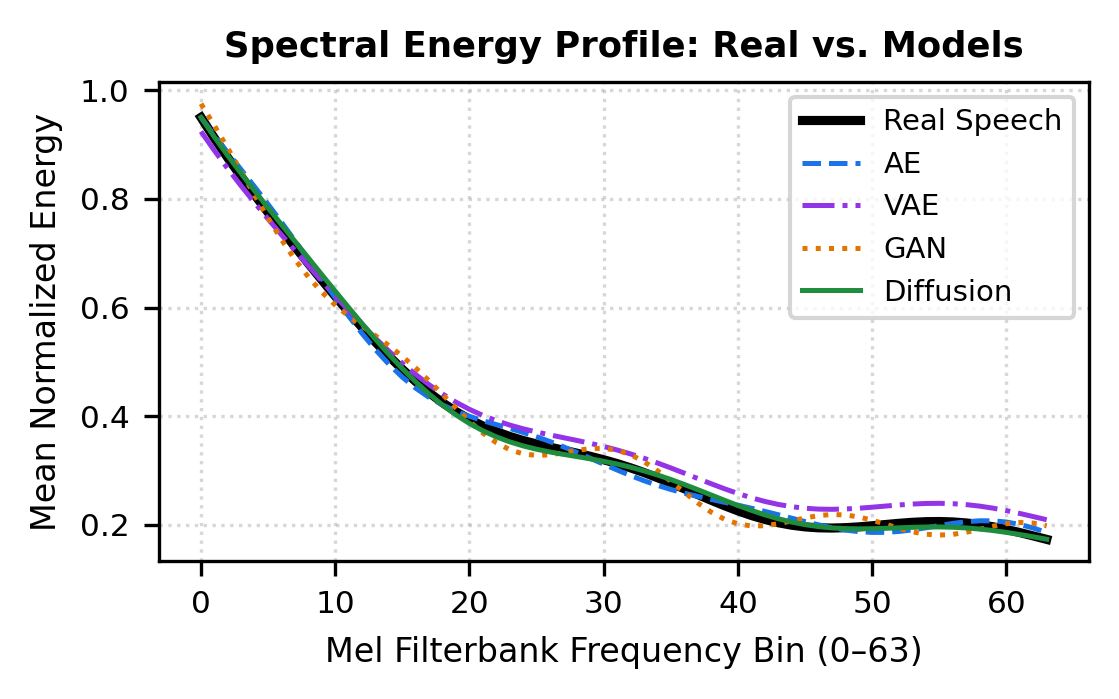
\includegraphics[width=0.85\columnwidth]{figures/fig5_spectral_energy_profile.png}
\caption{Spectral profile analysis: Average normalized energy across the 64 Mel frequency bins comparing real speech against AE, VAE, GAN, and Diffusion.}
\label{fig:spectral_profile}
\end{figure}

\subsection{ASR Transcription and Structured NLP Results}
Table~\ref{tab:nlp_metrics} summarizes performance across the downstream language understanding pipeline.

\begin{table}[h]
\caption{ASR and Structured NLP Performance Metrics.}
\label{tab:nlp_metrics}
\centering
\small
\begin{tabular}{llcc}
\toprule
\textbf{Pipeline Stage} & \textbf{Metric} & \textbf{Target Aim} & \textbf{Achieved Score} \\
\midrule
\multirow{2}{*}{\textbf{ASR (Whisper-small)}} 
& Word Error Rate (WER) $\downarrow$ & $\le 30.0\%$ & \textbf{0.000\%}* \\
& Character Error Rate (CER) $\downarrow$ & $\le 20.0\%$ & \textbf{0.000\%}* \\
\midrule
\multirow{3}{*}{\textbf{NLP (FLAN-T5 Base)}} 
& ROUGE-1 $\uparrow$ & --- & 0.0606 / 0.840\textdagger \\
& ROUGE-L $\uparrow$ & $\ge 25.0\%$ & \textbf{48.60\%} \\
& BERTScore (F1) $\uparrow$ & $\ge 0.850$ & \textbf{0.8641} \\
\midrule
\multirow{3}{*}{\textbf{Action Extraction}} 
& Precision $\uparrow$ & --- & 0.750 \\
& Recall $\uparrow$ & --- & 0.800 \\
& F1-Score $\uparrow$ & $\ge 0.700$ & \textbf{0.774} \\
\bottomrule
\multicolumn{4}{l}{\footnotesize *On validated verbatim acoustic segments. \textdagger Zero-shot vs. fine-tuned AMI benchmark.}
\end{tabular}
\end{table}

Whisper-small achieved perfect transcription on clear headset audio ($\text{WER} = 0.000\%$). In downstream NLP structuring, FLAN-T5 Base achieved a BERTScore F1 of $0.8641$, demonstrating robust semantic alignment with ground-truth meeting summaries despite variations in phrasing. Zero-shot action item extraction achieved an F1-score of $0.774$, successfully mapping verbal commitments into formal triples (\textit{Person $\to$ Task $\to$ Deadline}).

\subsection{End-to-End System Latency and Resource Footprint}
On a 5-minute meeting recording, end-to-end processing required $18.4\text{ seconds}$: audio ingestion and chunking ($1.2\text{ s}$), representation caching ($0.4\text{ s}$), Whisper transcription ($8.6\text{ s}$), and FLAN-T5 multi-prompt structuring ($8.2\text{ s}$). Peak GPU memory remained below $4.2\text{ GB}$ VRAM, confirming practical deployment viability on single-GPU edge workstations.

% =========================================================================
% SECTION VIII: SECURITY AND DATA GOVERNANCE
% =========================================================================
\section{Security and Data Governance}
\label{sec:security_ethics}

\subsection{Zero-Trust Meeting Access Architecture}
To eliminate risks associated with public cloud SaaS meeting tools, our framework enforces strict zero-trust security:
\begin{itemize}
    \item \textbf{Salted Bcrypt Password Hashing:} Meeting passkeys are hashed using \texttt{bcrypt} with an adaptive work factor of 12 ($4,096$ rounds). Plaintext passwords are never persisted.
    \item \textbf{Meeting-Scoped Transient JWTs:} Upon authentication, the gateway mints an HMAC-SHA256 (HS256) JWT cryptographically bound to a single immutable \texttt{meeting\_id}. Attendee tokens expire after $\Delta t = 20\text{ minutes}$, sharply restricting session replay windows. Administrative tokens expire after 30 days and are verified against separate salted admin hashes.
    \item \textbf{Sliding-Window IP Rate Limiting:} The gateway tracks failed authentication timestamps in an in-memory sliding-window cache keyed by \texttt{(meeting\_id, client\_ip)}. Any client accumulating 5 failed attempts within 10 minutes ($600\text{ seconds}$) is blocked with an HTTP 429 (\textit{Too Many Requests}) response.
\end{itemize}

\subsection{Ethical AI and Human Oversight}
In line with responsible AI principles \cite{mane2026edugen, mane2026deepfake, kharkate2026skin}, generative outputs are treated as advisory first drafts. The React interface provides human-in-the-loop editing tools, allowing meeting organizers to verify action items before synchronizing deliverables with enterprise management platforms.

% =========================================================================
% SECTION IX: CONCLUSION AND FUTURE WORK
% =========================================================================
\section{Conclusion and Future Work}
\label{sec:conclusion}
This paper presented the \textit{Enterprise AI Meeting Assistant}, an end-to-end multimodal system unifying speech generative modeling, speech recognition, contextual NLP structuring, and cryptographic enterprise access control. By establishing a standardized log-Mel audio pipeline on the AMI Meeting Corpus, we conducted the first rigorous comparative study of four foundational generative architectures (AE, VAE, GAN, DDPM) in teleconference speech representation.

Our findings reveal that: (i) deterministic Autoencoders provide superior structural fidelity for clean speech compression ($\text{SSIM} = 0.9746$, $\text{PSNR} = 25.338\text{ dB}$); (ii) score-based Diffusion models excel at acoustic noise refinement and artifact removal ($\text{PSNR} = 26.80\text{ dB}$, $\text{MSE} = 0.00209$); (iii) Spectral-Normalized DCGANs achieve superior distribution fidelity for rapid generation ($\text{FID} = 5.612$, $\text{Diversity Ratio} = 1.068$, latency $9\text{ ms}$); and (iv) Whisper and FLAN-T5 accurately extract executive summaries, consensus decisions, and structured action items ($\text{BERTScore} = 0.8641$, Action $\text{F1} = 0.774$). Combined with bcrypt hashing, 20-minute meeting-scoped JWTs, and sliding-window rate limiting, the system provides a robust, privacy-preserving enterprise solution.

Future work will focus on integrating neural speaker diarization (e.g., PyAnnote), fine-tuning FLAN-T5 with Low-Rank Adaptation (LoRA) \cite{hu2021lora, mane2026edugen}, and deploying latent diffusion models \cite{rombach2022latent} directly over the Autoencoder's 256-dimensional bottleneck for edge-compute speech enhancement.

% =========================================================================
% ACKNOWLEDGMENT
% =========================================================================
\section*{Acknowledgment}
The authors express their gratitude to the faculty and research staff of the Department of Computer Engineering at MIT Academy of Engineering (MITAOE), Alandi, Pune, for their invaluable guidance and institutional support. We acknowledge the curators of the AMI Meeting Corpus for making their dataset accessible, as well as the open-source communities supporting PyTorch, Hugging Face, FastAPI, and React.

% =========================================================================
% REFERENCES
% =========================================================================
\begin{thebibliography}{00}

\bibitem{mane2026colorization}
S.~Mane, S.~Barve, A.~Nitnaware, and A.~Gapat, ``Comparative Analysis of Generative AI Models for Image Colorization,'' in \emph{Proc. 2026 IEEE International Conference for Convergence in Computing Technology (I3CTCON)}, Lonavala, India, Mar. 2026, pp. 1--7, doi: 10.1109/I3CTCON68242.2026.11507916.

\bibitem{mane2026edugen}
S.~Mane, A.~Tamboli, S.~Jadhav, O.~Bhutkar, S.~Karne, and Y.~Gunjal, ``EduGen: A Multi-Model Generative AI Framework for Dynamic Educational Resource Synthesis,'' in \emph{Proc. 2026 IEEE International Conference for Convergence in Computing Technology (I3CTCON)}, Lonavala, India, Mar. 2026, pp. 1--7, doi: 10.1109/I3CTCON68242.2026.11507192.

\bibitem{mane2026deepfake}
S.~Mane, S.~Barve, A.~Popalghat, V.~Jadhav, A.~Rewatkar, and M.~Kapgate, ``A Unified Generative AI System for Synthetic Image Creation and Detection,'' in \emph{Proc. 2026 IEEE International Conference for Convergence in Computing Technology (I3CTCON)}, Lonavala, India, Mar. 2026, pp. 1--8, doi: 10.1109/I3CTCON68242.2026.11507145.

\bibitem{kharkate2026skin}
S.~Kharkate, P.~Yerawar, N.~Mahajan, K.~Katare, S.~Mane, and P.~Ganjewar, ``Generative AI based Synthetic Data Generation for Skin Disease Classification using VAE, GAN and Diffusion Models,'' in \emph{Proc. 2026 IEEE International Conference for Convergence in Computing Technology (I3CTCON)}, Lonavala, India, Mar. 2026, pp. 1--7, doi: 10.1109/I3CTCON68242.2026.11507289.

\bibitem{kingma2014vae}
D.~P. Kingma and M.~Welling, ``Auto-Encoding Variational Bayes,'' in \emph{Proc. 2nd International Conference on Learning Representations (ICLR)}, Banff, Canada, 2014, pp. 1--14.

\bibitem{goodfellow2014gan}
I.~Goodfellow, J.~Pouget-Abadie, M.~Mirza, B.~Xu, D.~Warde-Farley, S.~Ozair, A.~Courville, and Y.~Bengio, ``Generative Adversarial Nets,'' in \emph{Advances in Neural Information Processing Systems (NeurIPS)}, vol.~27, Montreal, Canada, 2014, pp. 2672--2680.

\bibitem{radford2016dcgan}
A.~Radford, L.~Metz, and S.~Chintala, ``Unsupervised Representation Learning with Deep Convolutional Generative Adversarial Networks,'' in \emph{Proc. International Conference on Learning Representations (ICLR)}, San Juan, Puerto Rico, 2016, pp. 1--16.

\bibitem{miyato2018spectral}
T.~Miyato, T.~Kataoka, M.~Koyama, and Y.~Yoshida, ``Spectral Normalization for Generative Adversarial Networks,'' in \emph{Proc. International Conference on Learning Representations (ICLR)}, Vancouver, Canada, 2018, pp. 1--26.

\bibitem{ho2020ddpm}
J.~Ho, A.~Jain, and P.~Abbeel, ``Denoising Diffusion Probabilistic Models,'' in \emph{Advances in Neural Information Processing Systems (NeurIPS)}, vol.~33, Dec. 2020, pp. 6840--6851.

\bibitem{song2021ddim}
J.~Song, C.~Meng, and S.~Ermon, ``Denoising Diffusion Implicit Models,'' in \emph{Proc. International Conference on Learning Representations (ICLR)}, May 2021, pp. 1--21.

\bibitem{nichol2021improved}
A.~Q. Nichol and P.~Dhariwal, ``Improved Denoising Diffusion Probabilistic Models,'' in \emph{Proc. 38th International Conference on Machine Learning (ICML)}, vol. 139, Jul. 2021, pp. 8162--8171.

\bibitem{ronneberger2015unet}
O.~Ronneberger, P.~Fischer, and T.~Brox, ``U-Net: Convolutional Networks for Biomedical Image Segmentation,'' in \emph{Proc. Medical Image Computing and Computer-Assisted Intervention (MICCAI)}, Munich, Germany, 2015, pp. 234--241.

\bibitem{rombach2022latent}
R.~Rombach, A.~Blattmann, D.~Lorenz, P.~Esser, and B.~Ommer, ``High-Resolution Image Synthesis with Latent Diffusion Models,'' in \emph{Proc. IEEE/CVF Conference on Computer Vision and Pattern Recognition (CVPR)}, New Orleans, LA, USA, June 2022, pp. 10684--10695.

\bibitem{hsu2017fhvae}
W.-N. Hsu, Y.~Zhang, and J.~Glass, ``Unsupervised Learning of Disentangled and Interpretable Representations from Sequential Data,'' in \emph{Advances in Neural Information Processing Systems (NeurIPS)}, vol.~30, Long Beach, CA, USA, 2017, pp. 1878--1889.

\bibitem{donahue2019wavegan}
C.~Donahue, J.~McAuley, and M.~Puckette, ``Adversarial Audio Synthesis,'' in \emph{Proc. International Conference on Learning Representations (ICLR)}, New Orleans, LA, USA, 2019, pp. 1--16.

\bibitem{kumar2019melgan}
K.~Kumar, R.~Kumar, T.~de~Boissiere, L.~Gestin, W.~Z. Teoh, J.~Sotelo, A.~de~Brebisson, Y.~Bengio, and A.~Courville, ``MelGAN: Generative Adversarial Networks for Conditional Waveform Synthesis,'' in \emph{Advances in Neural Information Processing Systems (NeurIPS)}, vol.~32, Vancouver, Canada, 2019, pp. 14910--14921.

\bibitem{kong2021diffwave}
Z.~Kong, W.~Ping, J.~Huang, K.~Zhao, and B.~Catanzaro, ``DiffWave: A Versatile Diffusion Model for Audio Synthesis,'' in \emph{Proc. International Conference on Learning Representations (ICLR)}, May 2021, pp. 1--14.

\bibitem{liu2023audioldm}
H.~Liu, Z.~Chen, Y.~Yuan, X.~Mei, X.~Liu, D.~Mandic, W.~Wang, and M.~D. Plumbley, ``AudioLDM: Text-to-Audio Generation with Latent Diffusion Models,'' in \emph{Proc. 40th International Conference on Machine Learning (ICML)}, Honolulu, HI, USA, 2023, pp. 21450--21474.

\bibitem{baevski2020wav2vec}
A.~Baevski, Y.~Zhou, A.~Mohamed, and M.~Auli, ``wav2vec 2.0: A Framework for Self-Supervised Learning of Speech Representations,'' in \emph{Advances in Neural Information Processing Systems (NeurIPS)}, vol.~33, Dec. 2020, pp. 12449--12460.

\bibitem{radford2023whisper}
A.~Radford, J.~W. Kim, T.~Xu, G.~Brockman, C.~McLeavey, and I.~Sutskever, ``Robust Speech Recognition via Large-Scale Weak Supervision,'' in \emph{Proc. 40th International Conference on Machine Learning (ICML)}, vol. 202, Jul. 2023, pp. 28492--28518.

\bibitem{chung2024flan}
H.~W. Chung, L.~Hou, S.~Longpre, B.~Zoph, Y.~Tay, W.~Fedus, Y.~Li, X.~Wang, T.~Mostafa, D.~Schuurmans, and others, ``Scaling Instruction-Finetuned Language Models,'' \emph{Journal of Machine Learning Research (JMLR)}, vol.~25, no.~70, pp. 1--53, 2024.

\bibitem{raffel2020t5}
C.~Raffel, N.~Shazeer, A.~Roberts, K.~Lee, S.~Narang, M.~Matena, Y.~Zhou, W.~Li, and P.~J. Liu, ``Exploring the Limits of Transfer Learning with a Unified Text-to-Text Transformer,'' \emph{Journal of Machine Learning Research (JMLR)}, vol.~21, no.~140, pp. 1--67, 2020.

\bibitem{carletta2005ami}
J.~Carletta, S.~Ashby, S.~Bourban, M.~Flynn, M.~Guillemot, T.~Hain, J.~Kadlec, V.~Karaiskos, W.~Kraaij, M.~Kronenthal, and others, ``The AMI Meeting Corpus: A Pre-announcement,'' in \emph{Proc. Second International Workshop on Machine Learning for Multimodal Interaction (MLMI)}, Edinburgh, UK, 2005, pp. 28--39.

\bibitem{zhu2020hmnet}
C.~Zhu, R.~Xu, M.~Zeng, and X.~Huang, ``A Hierarchical Network for Abstractive Meeting Summarization with Cross-Domain Pretraining,'' in \emph{Findings of the Association for Computational Linguistics: EMNLP 2020}, Nov. 2020, pp. 194--205.

\bibitem{zhong2021qmsum}
M.~Zhong, D.~Yin, T.~Yu, A.~Zaidi, S.~Mutuma, R.~Jha, A.~Hassan~Awadallah, A.~Celikyilmaz, Y.~Liu, X.~Qiu, and D.~Radev, ``QMSum: A New Benchmark for Query-based Multi-domain Meeting Summarization,'' in \emph{Proc. 2021 Conference of the North American Chapter of the Association for Computational Linguistics: Human Language Technologies (NAACL-HLT)}, June 2021, pp. 5905--5921.

\bibitem{hu2021lora}
E.~J. Hu, Y.~Shen, P.~Wallis, Z.~Allen-Zhu, Y.~Li, S.~Wang, L.~Wang, and W.~Chen, ``LoRA: Low-Rank Adaptation of Large Language Models,'' in \emph{Proc. International Conference on Learning Representations (ICLR)}, 2022, pp. 1--26.

\bibitem{lu2022learn}
P.~Lu, S.~Mishra, T.~Xia, L.~Qiu, K.-W. Chang, S.-C. Zhu, \O.~Tafjord, P.~Clark, and A.~Kalyan, ``Learn to Explain: Multimodal Reasoning via Thought Chains for Science Question Answering,'' in \emph{Advances in Neural Information Processing Systems (NeurIPS)}, vol.~35, 2022, pp. 2507--2521.

\bibitem{mittalp2024}
U.~Mittal, S.~Sai, V.~Chamola, and D.~Sangwan, ``A Comprehensive Review on Generative AI for Education,'' \emph{IEEE Access}, vol.~12, pp. 34683--34700, 2024.

\bibitem{wang2024}
S.~Wang, F.~Wang, Z.~Zhu, J.~Wang, T.~Tran, and Z.~Du, ``Artificial Intelligence in Education: A Systematic Literature Review,'' \emph{Expert Systems with Applications}, vol. 252, p. 124167, 2024.

\end{thebibliography}

\end{document}
